\chapter{Eigen value problems/solutions}
\begin{abox}
	Practice set 1 solutions
	\end{abox}
\begin{enumerate}
	\begin{minipage}{\textwidth}
	\item The energy of the first excited quantum state of a particle in the two-dimensional potential $V(x, y)=\frac{1}{2} m \omega^{2}\left(x^{2}+4 y^{2}\right)$ is
	\exyear{NET DEC 2011}
\end{minipage}
\begin{tasks}(2)
	\task[\textbf{A.}] $2 \hbar \omega$
	\task[\textbf{B.}]$3 \hbar \omega$
	\task[\textbf{C.}]$\frac{3}{2} \hbar \omega$
	\task[\textbf{D.}] $\frac{5}{2} \hbar \omega$
\end{tasks}
\begin{answer}
	$V(x, y)=\frac{1}{2} m \omega^{2}\left(x^{2}+4 y^{2}\right)=\frac{1}{2} m \omega^{2} x^{2}+\frac{1}{2} m 4 \omega^{2} y^{2}, \\
	E=\left(n_{x}+\frac{1}{2}\right) \hbar \omega+\left(n_{y}+\frac{1}{2}\right) 2 \hbar \omega$\\
	For ground state energy $n_{x}=0, n_{y}=0 \Rightarrow E=\frac{\hbar \omega}{2}+\frac{1}{2} 2 \hbar \omega=\frac{3 \hbar \omega}{2}$\\
	First exited state energy $n_{x}=1, n_{y}=0 \Rightarrow \frac{3 \hbar \omega}{2}+\hbar \omega=\frac{5 \hbar \omega}{2}$\\
	The correct option is \textbf{(d)}
\end{answer}
\begin{minipage}{\textwidth}
	\item Let $|0\rangle$ and $|1\rangle$ denote the normalized eigenstates corresponding to the ground and first excited states of a one dimensional harmonic oscillator. The uncertainty $\Delta p$ in the state $\frac{1}{\sqrt{2}}(|0\rangle+|1\rangle)$, is
	\exyear{NET DEC 2011}
\end{minipage}
\begin{tasks}(2)
	\task[\textbf{A.}] $\Delta p=\sqrt{\hbar m \omega} / 2$
	\task[\textbf{B.}]$\Delta p=\sqrt{\hbar m \omega / 2}$
	\task[\textbf{C.}]$\Delta p=\sqrt{\hbar m \omega}$
	\task[\textbf{D.}]$\Delta p=\sqrt{2 \hbar m \omega}$
\end{tasks}
\begin{answer}
	$\begin{aligned}
	&\text { Solution: }|\psi\rangle=\frac{1}{\sqrt{2}}(|0\rangle+|1\rangle), p=i \sqrt{\frac{m \omega \hbar}{2}}\left(a^{\dagger}-a\right) \\
	&\begin{aligned}
	a^{\dagger}|\psi\rangle &=\frac{1}{\sqrt{2}}(\sqrt{1}|1\rangle+\sqrt{2}|2\rangle) \text { and } a|\psi\rangle=\frac{1}{\sqrt{2}}(0+\sqrt{1}|0\rangle) \\
	\langle p\rangle &=i \sqrt{\frac{m \omega \hbar}{2}}\left(\left\langle\psi\left|a^{\dagger}-a\right| \psi\right\rangle\right)=0, p^{2}=-\frac{m \omega \hbar}{2}\left(a^{\dagger^{2}}+a^{2}-(2 N+1)\right) \\
	\left\langle p^{2}\right\rangle &=\frac{-m \omega \hbar}{2}\left[\left\langle a^{+^{2}}\right\rangle+\left\langle a^{2}\right\rangle-\langle 2 N+1\rangle\right]=\frac{m \omega \hbar}{2}\langle 2 N+1\rangle=\frac{m \omega \hbar}{2}\left(2 \cdot \frac{1}{2}+1\right)=m \omega \hbar \\
	\Delta p &=\sqrt{\left\langle p^{2}\right\rangle-\langle p\rangle^{2}}=\sqrt{m \omega \hbar}
	\end{aligned}
	\end{aligned}$\\
	The correct option is \textbf{(c)}	
\end{answer}
\begin{minipage}{\textwidth}
	\item A particle of mass $m$ is in a cubic box of size $a$. The potential inside the box $(0 \leq x<a, 0 \leq y<a, 0 \leq z<a)$ is zero and infinite outside. If the particle is in an eigenstate of energy $E=\frac{14 \pi^{2} \hbar^{2}}{2 m a^{2}}$, its wavefunction is
	\exyear{NET JUNE 2012}
\end{minipage}
\begin{tasks}(2)
	\task[\textbf{A.}] $\psi=\left(\frac{2}{a}\right)^{3 / 2} \sin \frac{3 \pi x}{a} \sin \frac{5 \pi y}{a} \sin \frac{6 \pi z}{a}$
	\task[\textbf{B.}] $\psi=\left(\frac{2}{a}\right)^{3 / 2} \sin \frac{7 \pi x}{a} \sin \frac{4 \pi y}{a} \sin \frac{3 \pi z}{a}$
	\task[\textbf{C.}]$\psi=\left(\frac{2}{a}\right)^{3 / 2} \sin \frac{4 \pi x}{a} \sin \frac{8 \pi y}{a} \sin \frac{2 \pi z}{a}$
	\task[\textbf{D.}]$\psi=\left(\frac{2}{a}\right)^{3 / 2} \sin \frac{\pi x}{a} \sin \frac{2 \pi y}{a} \sin \frac{3 \pi z}{a}$
\end{tasks}
\begin{answer}
	$E_{n_{x}, n_{y}, n_{z}}=\left(n_{x}^{2}+n_{y}^{2}+n_{z}^{2}\right) \frac{\pi^{2} \hbar^{2}}{2 m a^{2}}=\frac{14 \pi^{2} \hbar^{2}}{2 m a^{2}}$ $\Rightarrow n_{x}^{2}+n_{y}^{2}+n_{z}^{2}=14 \Rightarrow n_{x}=1, n_{y}=2, n_{z}=3 .$\\
	The correct option is \textbf{(d)}	
\end{answer}
\begin{minipage}{\textwidth}
	\item $\text { A particle in one-dimension is in the potential }$
	$V(x)=\left\{\begin{array}{llll}
	\infty & , & \text { if } & x<0 \\
	-V_{0} & , & \text { if } & 0 \leq x \leq l \\
	0 & & \text { if } & x>l
	\end{array}\right.$
	$\text { If there is at least one bound state, the minimum depth of potential is }$
	\exyear{NET JUNE 2012}
\end{minipage}
\begin{tasks}(2)
	\task[\textbf{A.}] $\frac{\hbar^{2} \pi^{2}}{8 m l^{2}}$
	\task[\textbf{B.}]$\frac{\hbar^{2} \pi^{2}}{2 m l^{2}}$
	\task[\textbf{C.}]$\frac{2 \hbar^{2} \pi^{2}}{m l^{2}}$
	\task[\textbf{D.}]$\frac{\hbar^{2} \pi^{2}}{m l^{2}}$
\end{tasks}
\begin{answer}
	\begin{figure}[H]
		\centering
		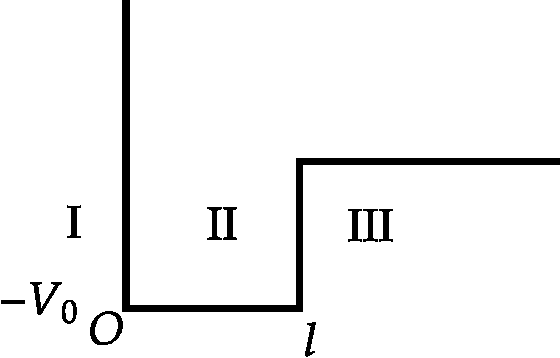
\includegraphics[height=3cm,width=5cm]{diagram-20210921(4)-crop}
		\caption{}
		\label{}
	\end{figure}
	For bound state, $-V_{0}<E<0$\\
	Wave function in region $\mathrm{I}, \psi_{I}=0, \psi_{I I}=A \sin k x+B \cos k x, \psi_{I I I}=c e^{-\gamma x}$ where $k=\frac{\sqrt{2 m\left(V_{0}+E\right)}}{\hbar^{2}}, \gamma=\frac{\sqrt{2 m(-E)}}{\hbar^{2}}$.\\
	Use Boundary condition at $x=0$ and $x=l$\\
	(wave function is continuous and differential at $x=0$ and $x=l$ ), one will get $k \cot k l=-\gamma \Rightarrow k l \cot k l=-\gamma l \Rightarrow \eta=-\xi \cot \xi$\\
	where $\gamma l=\eta, k l=\xi$.\\
	$\Rightarrow \eta^{2}+\xi^{2}=\frac{2 m V_{0} l^{2}}{\hbar^{2}}$\\
	$\text { For one bound state }\left(\frac{2 m V_{0} l^{2}}{\hbar^{2}}\right)^{1 / 2}=\frac{\pi}{2} \Rightarrow V_{0}=\frac{\pi^{2} \hbar^{2}}{8 m l^{2}} \text {. }$\\
	\begin{figure}[H]
		\centering
		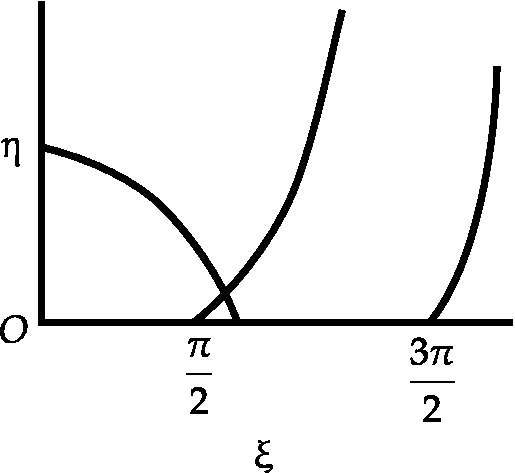
\includegraphics[height=3cm,width=5cm]{diagram-20210921(3)-crop}
		\caption{}
		\label{}
	\end{figure}
	The correct option is \textbf{(a)}	
\end{answer}
\begin{minipage}{\textwidth}
	\item $\text { The energy eigenvalues of a particle in the potential } V(x)=\frac{1}{2} m \omega^{2} x^{2}-a x \text { are }$
	\exyear{NET DEC 2012}
\end{minipage}
\begin{tasks}(2)
	\task[\textbf{A.}] $E n=\left(n+\frac{1}{2}\right) \hbar \omega-\frac{a^{2}}{2 m \omega^{2}}$
	\task[\textbf{B.}]$E n=\left(n+\frac{1}{2}\right) \hbar \omega+\frac{a^{2}}{2 m \omega^{2}}$
	\task[\textbf{C.}]$E n=\left(n+\frac{1}{2}\right) \hbar \omega-\frac{a^{2}}{m \omega^{2}}$
	\task[\textbf{D.}]$E n=\left(n+\frac{1}{2}\right) \hbar \omega$
\end{tasks}
\begin{answer}
	Hamiltonian $(H)$ of Harmonic oscillator, $H=\frac{p_{x}^{2}}{2 m}+\frac{1}{2} m \omega^{2} x^{2}$\\
	Eigenvalue of this, $E_{n}=\left(n+\frac{1}{2}\right) \hbar \omega$\\
	But here, $H=\frac{p_{x}^{2}}{2 m}+\frac{1}{2} m \omega^{2} x^{2}-a x \Rightarrow H=\frac{p_{x}^{2}}{2 m}+\frac{1}{2} m \omega^{2}\left[x^{2}-\frac{2 a x}{m \omega^{2}}+\frac{a^{2}}{m^{2} \omega^{4}}\right]-\frac{a^{2}}{2 m \omega^{2}}$\\
	$H=\frac{p_{x}^{2}}{2 m}+\frac{1}{2} m \omega^{2}\left[x-\frac{a}{m \omega^{2}}\right]^{2}-\frac{a^{2}}{2 m \omega^{2}}$\\
	Energy eigenvalue, $E_{n}=\left(n+\frac{1}{2}\right) \hbar \omega-\frac{a^{2}}{2 m \omega^{2}}$\\
	The correct option is \textbf{(a)}	
\end{answer}
\begin{minipage}{\textwidth}
	\item A particle is in the ground state of an infinite square well potential is given by,
	$$
	V(x)= \begin{cases}0 & \text { for }-a \leq x \leq a \\ \infty & \text { otherwise }\end{cases}
	$$
	The probability to find the particle in the interval between $-\frac{a}{2}$ and $\frac{a}{2}$ is
	\exyear{NET DEC 2013}
\end{minipage}
\begin{tasks}(2)
	\task[\textbf{A.}] $\frac{1}{2}$ 
	\task[\textbf{B.}]$\frac{1}{2}+\frac{1}{\pi}$
	\task[\textbf{C.}]$\frac{1}{2}-\frac{1}{\pi}$
	\task[\textbf{D.}]$\frac{1}{\pi}$
\end{tasks}
\begin{answer}
	The probability to find the particle in the interval between $-\frac{a}{2}$ and $\frac{a}{2}$ is
	$$
	\begin{aligned}
	&=\int_{-a / 2}^{a / 2} \sqrt{\frac{2}{2 a}} \cdot \sqrt{\frac{2}{2 a}} \cos \frac{\pi x}{2 a} \cdot \cos \frac{\pi x}{2 a} d x=\int_{-a / 2}^{a / 2} \frac{1}{a} \cos ^{2} \frac{\pi x}{2 a} d x=\frac{1}{a} \times \frac{1}{2}\left[\int_{-a / 2}^{a / 2}\left(1+\cos \frac{2 \pi x}{2 a}\right) d x\right] \\
	&=\frac{1}{2 a}\left[x+\frac{a}{\pi} \sin \frac{\pi x}{a}\right]_{-a / 2}^{a / 2}=\frac{1}{2 a}\left[\frac{a}{2}+\frac{a}{2}+\frac{a}{\pi}(1+1)\right]=\frac{1}{2 a}\left[a+\frac{2 a}{\pi}\right]=\left(\frac{1}{2}+\frac{1}{\pi}\right)
	\end{aligned}
	$$
	The correct option is \textbf{(b)}
\end{answer}
\begin{minipage}{\textwidth}
	\item A particle of mass $m$ in the potential $V(x, y)=\frac{1}{2} m \omega^{2}\left(4 x^{2}+y^{2}\right)$, is in an eigenstate of energy $E=\frac{5}{2} \hbar \omega$. The corresponding un-normalized eigen function is
	\exyear{NET JUNE 2014}
\end{minipage}
\begin{tasks}(2)
	\task[\textbf{A.}] $y \exp \left[-\frac{m \omega}{2 \hbar}\left(2 x^{2}+y^{2}\right)\right]$
	\task[\textbf{B.}]$x \exp \left[-\frac{m \omega}{2 \hbar}\left(2 x^{2}+y^{2}\right)\right]$
	\task[\textbf{C.}]$y \exp \left[-\frac{m \omega}{2 \hbar}\left(x^{2}+y^{2}\right)\right]$
	\task[\textbf{D.}]$x y \exp \left[-\frac{m \omega}{2 \hbar}\left(x^{2}+y^{2}\right)\right]$
\end{tasks}
\begin{answer}
	$V(x, y)=\frac{1}{2} m \omega^{2}\left(4 x^{2}+y^{2}\right), E=\frac{5}{2} \hbar \omega$\\
	$\begin{aligned}
	&\Rightarrow V(x, y)=\frac{1}{2} m(2 \omega)^{2} x^{2}+\frac{1}{2} m \omega^{2} y^{2} \\
	&\text { Now, } E_{n}=\left(n_{x}+\frac{1}{2}\right) \hbar \omega_{x}+\left(n_{y}+\frac{1}{2}\right) \hbar \omega_{y}=\left(n_{x}+\frac{1}{2}\right) 2 \hbar \omega+\left(n_{y}+\frac{1}{2}\right) \hbar \omega \\
	&\Rightarrow E_{n}=\left(2 n_{x}+n_{y}+\frac{3}{2}\right) \hbar \omega \\
	&\because E_{n}=\frac{5}{2} \hbar \omega \text { when } n_{x}=0 \text { and } n_{y}=1 .
	\end{aligned}$\\
	The correct option is \textbf{(a)}
\end{answer}
\begin{minipage}{\textwidth}
	\item A particle of mass $m$ in three dimensions is in the potential
	$$
	V(r)= \begin{cases}0, & r<a \\ \infty, & r>a\end{cases}
	$$
	Its ground state energy is
	\exyear{NET JUNE 2014}
\end{minipage}
\begin{tasks}(2)
	\task[\textbf{A.}] $\frac{\pi^{2} \hbar^{2}}{2 m a^{2}}$
	\task[\textbf{B.}]$\frac{\pi^{2} \hbar^{2}}{m a^{2}}$
	\task[\textbf{C.}]$\frac{3 \pi^{2} \hbar^{2}}{2 m a^{2}}$
	\task[\textbf{D.}]$\frac{9 \pi^{2} \hbar^{2}}{2 m a^{2}}$
\end{tasks}
\begin{answer}
	$\left(-\frac{\hbar^{2}}{2 m}\right) \frac{d^{2} u(r)}{d r^{2}}+\frac{l(l+1)}{2 m r^{2}}+V(r) u(r)=E u(r)$ $\frac{d^{2} u(r)}{d r^{2}}=-K^{2} u(r) $\\
	$\because K=\sqrt{\frac{2 m E}{\hbar^{2}}}, l=0, V(r)=0$ $u(r)=A \sin K r+B \cos K r$\\
	Using boundary condition, $B=0$,\\
	$u(r)=A \sin K r, r=a, u(r)=0 \Rightarrow \sin K a=0 \Rightarrow K a=n \pi \Rightarrow E=\frac{\pi^{2} \hbar^{2}}{2 m a^{2}} \quad \because n=1$	
\end{answer}
\begin{minipage}{\textwidth}
	\item A particle in the infinite square well potential
	$$
	V(x)= \begin{cases}0 & , 0<x<a \\ \infty & \text { otherwise }\end{cases}
	$$
	is prepared in a state with the wavefunction
	$$
	\psi(x)= \begin{cases}A \sin ^{3}\left(\frac{\pi x}{a}\right), & 0<x<a \\ 0 & \text { otherwise }\end{cases}
	$$
	The expectation value of the energy of the particle is
	\exyear{NET JUNE 2014}
\end{minipage}
\begin{tasks}(2)
	\task[\textbf{A.}] $\frac{5 \hbar^{2} \pi^{2}}{2 m a^{2}}$
	\task[\textbf{B.}]$\frac{9 \hbar^{2} \pi^{2}}{2 m a^{2}}$
	\task[\textbf{C.}]$\frac{9 \hbar^{2} \pi^{2}}{10 m a^{2}}$
	\task[\textbf{D.}]$\frac{\hbar^{2} \pi^{2}}{2 m a^{2}}$
\end{tasks}
\begin{answer}
	$ V(x)=\left\{\begin{array}{ll}
	0, & 0<x<a \\
	\infty, & \text { otherwise }
	\end{array} \quad \psi(x)=\left\{\begin{array}{ll}
	A \sin ^{3}\left(\frac{\pi x}{a}\right), & 0<x<a \\
	0 & \text { otherwise }
	\end{array}\right\}\right.$\\
	$\begin{aligned}
	\psi(x) &=A \sin ^{3}\left(\frac{\pi x}{a}\right)=A \frac{3}{4} \sin \frac{\pi x}{a}-A \frac{1}{4} \sin \frac{3 \pi x}{a} \quad\left(\because \sin 3 A=3 \sin A-4 \sin ^{3} A\right) \\
	&=\frac{A}{4}\left[\sqrt{\frac{a}{2}} \sqrt{\frac{2}{a}} \times 3 \sin \frac{\pi x}{a}-\sqrt{\frac{a}{2}} \sqrt{\frac{2}{a}} \sin \frac{3 \pi x}{a}\right] \Rightarrow \psi(x)=\frac{A}{4}\left[3 \sqrt{\frac{a}{2}} \phi_{1}(x)-\sqrt{\frac{a}{2}} \phi_{3}(x)\right] \\
	\langle\psi \mid \psi\rangle &=1 \Rightarrow 9 \frac{a}{32} A^{2}+\frac{a}{32} A^{2}=1 \Rightarrow \frac{10 a}{32} A^{2}=1 \Rightarrow A=\sqrt{\frac{32}{10 a}} \\
	\psi(x) &=\frac{1}{4}\left(3 \cdot \sqrt{\frac{a}{2}} \sqrt{\frac{32}{10 a}} \phi_{1}(x)-\sqrt{\frac{a}{2}} \sqrt{\frac{32}{10 a}} \phi_{3}(x)\right)=\frac{3}{\sqrt{10}} \phi_{1}(x)-\frac{1}{\sqrt{10}} \phi_{3}(x)
	\end{aligned}$\\
	Now, $\quad E_{1}=\frac{\pi^{2} \hbar^{2}}{2 m a^{2}}, \quad E_{3}=\frac{9 \pi^{2} \hbar^{2}}{2 m a^{2}} \Rightarrow\langle E\rangle=a_{n} P\left(a_{n}\right)$
	Probability $P\left(E_{1}\right)=\frac{\left\langle\left.\left\langle\varphi_{1} \mid \psi\right\rangle\right|^{2}\right.}{\langle\psi \mid \psi\rangle}=\frac{9}{10}, P\left(E_{3}\right)=\frac{\left|\left\langle\phi_{2} \mid \psi\right\rangle\right|^{2}}{\langle\psi \mid \psi\rangle}=\frac{1}{10}$
	$\langle E\rangle=\frac{9}{10} \times \frac{\pi^{2} \hbar^{2}}{2 m a^{2}}+\frac{1}{10} \times \frac{9 \pi^{2} \hbar^{2}}{2 m a^{2}} \Rightarrow\langle E\rangle=\frac{9 \pi^{2} \hbar^{2}}{10 m a^{2}}$\\
	The correct option is \textbf{(c)}
\end{answer}
\begin{minipage}{\textwidth}
	\item The ground state energy of the attractive delta function potential
	$$
	V(x)=-b \delta(x),
	$$
	where $b>0$, is calculated with the variational trial function
	$$
	\psi(x)=\left\{\begin{array}{ccc}
	A \cos \frac{\pi x}{2 a}, & \text { for } & -a<x<a, \\
	0, & & \text { otherwise, }
	\end{array}\right\} \text { is }
	$$
	\exyear{NET DEC 2014}
\end{minipage}
\begin{tasks}(2)
	\task[\textbf{A.}] $-\frac{m b^{2}}{\pi^{2} \hbar^{2}}$
	\task[\textbf{B.}]$-\frac{2 m b^{2}}{\pi^{2} \hbar^{2}}$
	\task[\textbf{C.}]$-\frac{m b^{2}}{2 \pi^{2} \hbar^{2}}$
	\task[\textbf{D.}]$-\frac{m b^{2}}{4 \pi^{2} \hbar^{2}}$
\end{tasks}
\begin{answer}
	$V(x)=-b \delta(x) ; \quad b>0 \quad \text { and } \quad \psi(x)=\left\{A \cos \frac{\pi x}{2 a} ; \quad-a<x<a\right.$\\
	Normalized $\psi=\sqrt{\frac{2}{2 a}} \cos \frac{\pi x}{2 a}$\\
	$\langle T\rangle=\int_{-a}^{a} \psi^{*}\left(\frac{-\hbar^{2}}{2 m}\right) \frac{\partial^{2}}{\partial x^{2}} \psi d x=\frac{\pi^{2} \hbar^{2}}{8 m a^{2}}$\\
	$\langle V\rangle=\int_{-a}^{a} \psi^{*}-b \delta(x) \psi d x=\frac{2}{2 a}(-b)=-\frac{b}{a}$\\
	$\langle E\rangle=\frac{\pi^{2} \hbar^{2}}{8 m a^{2}}-\frac{b}{a} \Rightarrow \frac{\partial\langle E\rangle}{\partial a}=\frac{-2 \pi^{2} \hbar^{2}}{8 m a^{3}}+\frac{b}{a^{2}}=0 \Rightarrow \frac{-\pi^{2} \hbar^{2}}{4 m a}+b=0 \Rightarrow a=\frac{\pi^{2} \hbar^{2}}{4 m b}$\\
	Put the value of $a$ in equation: $\langle E\rangle=\frac{\pi^{2} \hbar^{2}}{8 m a^{2}}-\frac{b}{a}=\frac{\pi^{2} \hbar^{2}(4 m b)^{2}}{8 m\left(\pi^{2} \hbar^{2}\right)^{2}}-\frac{b(4 m b)}{\left(\pi^{2} \hbar^{2}\right)}=-\frac{2 m b^{2}}{\pi^{2} \hbar^{2}}$\\
	The correct option is \textbf{(b)}
\end{answer}
\begin{minipage}{\textwidth}
	\item Let $|\psi\rangle=c_{0}|0\rangle+c_{1}|1\rangle$ (where $c_{0}$ and $c_{1}$ are constants with $c_{0}^{2}+c_{1}^{2}=1$ ) be a linear combination of the wavefunctions of the ground and first excited states of the onedimensional harmonic oscillator. For what value of $c_{0}$ is the expectation value $\langle x\rangle$ a maximum?
	\exyear{NET DEC 2014}
\end{minipage}
\begin{tasks}(2)
	\task[\textbf{A.}] $\langle x\rangle=\sqrt{\frac{\hbar}{m \omega}}, \quad c_{0}=\frac{1}{\sqrt{2}}$
	\task[\textbf{B.}]$\langle x\rangle=\sqrt{\frac{\hbar}{2 m \omega}}, \quad c_{0}=\frac{1}{2}$
	\task[\textbf{C.}]$\langle x\rangle=\sqrt{\frac{\hbar}{2 m \omega}}, \quad c_{0}=\frac{1}{\sqrt{2}}$
	\task[\textbf{D.}]$\langle x\rangle=\sqrt{\frac{\hbar}{m \omega}}, \quad c_{0}=\frac{1}{2}$
\end{tasks}
\begin{answer}
	$\begin{aligned}
	&|\psi\rangle=c_{0}|0\rangle+c_{1}|1\rangle \\
	&\qquad \begin{array}{l}
	\langle X\rangle=\langle\psi|X| \psi\rangle \\
	\Rightarrow\langle X\rangle=2 c_{0} c_{1}\langle 0|X| 1\rangle=\left[\left(c_{0}^{2}+c_{1}^{2}\right)-\left(c_{0}-c_{1}\right)^{2}\right]\langle 0|X| 1\rangle=\left[1-\left(c_{0}-c_{1}\right)^{2}\right]\langle 0|X| 1\rangle \\
	\text { For max } \quad\langle X\rangle=c_{0}=c_{1} \quad \quad \because c_{0}^{2}+c_{1}^{2}=1 \Rightarrow c_{0}=\frac{1}{\sqrt{2}} \\
	\Rightarrow\langle X\rangle=2 \frac{1}{\sqrt{2}} \frac{1}{\sqrt{2}}\langle 0|X| 1\rangle=\langle 0|X| 1\rangle \\
	\sqrt{\frac{\hbar}{2 m \omega}}\left(\left\langle 0\left|a+a^{+}\right| 1\right\rangle\right) \Rightarrow\langle X\rangle=\sqrt{\frac{\hbar}{2 m \omega}}
	\end{array}
	\end{aligned}$\\
	The correct option is \textbf{(C)}
\end{answer}
\begin{minipage}{\textwidth}
	\item The ratio of the energy of the first excited state $E_{1}$, to that of the ground state $E_{0}$, to that of a particle in a three-dimensional rectangular box of side $L, L$ and $\frac{L}{2}$, is
	\exyear{NET JUNE 2015}
\end{minipage}
\begin{tasks}(2)
	\task[\textbf{A.}] $3: 2$
	\task[\textbf{B.}]$2: 1$
	\task[\textbf{C.}]$4: 1$
	\task[\textbf{D.}]$4: 3$
\end{tasks}
\begin{answer}
	$E=\frac{\pi^{2} \hbar^{2}}{2 m L^{2}}\left[n_{x}^{2}+n_{y}^{2}+4 n_{z}^{2}\right]$, for ground state $n_{x}=1, n_{y}=1, n_{z}=1 \Rightarrow E_{0}=\frac{6 \pi^{2} \hbar^{2}}{2 m L^{2}}$\\
	For first excited state $n_{x}=1, n_{y}=2, n_{z}=1 \Rightarrow E=E_{1}=\frac{\pi^{2} \hbar^{2}}{2 m L^{2}}(1+4+4)=\frac{9 \pi^{2} \hbar^{2}}{2 m L^{2}}$
	$\therefore \frac{E_{1}}{E_{0}}=\frac{9}{6}=\frac{3}{2}$\\
	The correct option is \textbf{(a)}
\end{answer}
\begin{minipage}{\textwidth}
	\item The ground state energy of a particle in potential $V(x)=g|x|$, estimated using the trail wavefunction\\
	$\psi(x)= \begin{cases}\sqrt{\frac{c}{a^{5}}}\left(a^{2}-x^{2}\right), & x<|a| \\ 0, & x \geq|a|\end{cases}$\\
	$\text { (where } g \text { and } c \text { are constants) is }$
	\exyear{NET DEC 2015}
\end{minipage}
\begin{tasks}(2)
	\task[\textbf{A.}] $\frac{15}{16}\left(\frac{\hbar^{2} g^{2}}{m}\right)^{1 / 3}$
	\task[\textbf{B.}]$\frac{5}{6}\left(\frac{\hbar^{2} g^{2}}{m}\right)^{1 / 3}$
	\task[\textbf{C.}] $\frac{3}{4}\left(\frac{\hbar^{2} g^{2}}{m}\right)^{1 / 3}$
	\task[\textbf{D.}] $\frac{7}{8}\left(\frac{\hbar^{2} g^{2}}{m}\right)^{1 / 3}$
\end{tasks}
\begin{answer}
	$\begin{aligned}
	&\text { on: } \int_{-a}^{a} \psi^{*} \psi d x=1 \Rightarrow c=\frac{15}{16} \\
	&\langle T\rangle=\frac{-\hbar^{2}}{2 m}\left(\frac{15}{16 a^{2}}\right) \int_{-a}^{a}\left(a^{2}-x^{2}\right) \frac{\partial^{2}}{\partial x^{2}}\left(a^{2}-x^{2}\right) d x \Rightarrow\langle T\rangle=\frac{10 \hbar^{2}}{4 m a^{2}} \\
	&\langle V\rangle=\frac{15 \times 2 g}{16 a^{5}} \int_{0}^{a} x\left(a^{2}-x^{2}\right) d x \Rightarrow\langle V\rangle=\frac{5}{16} g a \\
	&E=\langle T\rangle+\langle V\rangle
	\end{aligned}$
	$$
	\begin{aligned}
	&E=\frac{10 \hbar^{2}}{4 m a^{2}}+\frac{5 g a}{16} \\
	&\frac{d E}{d a}=0 \Rightarrow a^{3}=\frac{8 \hbar}{m g} \Rightarrow a=2\left(\frac{\hbar^{2}}{m g}\right)^{\frac{1}{3}}
	\end{aligned}
	$$
	put the value of $a$ in equation (i)
	$$
	E=\frac{15}{16}\left(\frac{\hbar^{2} g^{2}}{m}\right)^{\frac{1}{3}}
	$$
	The correct option is \textbf{(a)}
\end{answer}
\begin{minipage}{\textwidth}
	\item The state of a particle of mass $m$ in a one dimensional rigid box in the interval 0 to $L$ is given by the normalized wavefunction $\psi(x)=\sqrt{\frac{2}{L}}\left(\frac{3}{5} \sin \left(\frac{2 \pi x}{L}\right)+\frac{4}{5} \sin \left(\frac{4 \pi x}{L}\right)\right)$. If its energy is measured the possible outcomes and the average value of energy are, respectively
	\exyear{NET JUNE 2016}
\end{minipage}
\begin{tasks}(2)
	\task[\textbf{A.}] $\frac{h^{2}}{2 m L^{2}}, \frac{2 h^{2}}{m L^{2}}$ and $\frac{73}{50} \frac{h^{2}}{m L^{2}}$
	\task[\textbf{B.}] $\frac{h^{2}}{8 m L^{2}}, \frac{h^{2}}{2 m L^{2}}$ and $\frac{19}{40} \frac{h^{2}}{m L^{2}}$
	\task[\textbf{C.}]$\frac{h^{2}}{2 m L^{2}}, \frac{2 h^{2}}{m L^{2}}$ and $\frac{19}{10} \frac{h^{2}}{m L^{2}}$
	\task[\textbf{D.}]$\frac{h^{2}}{8 m L^{2}}, \frac{2 h^{2}}{m L^{2}}$ and $\frac{73}{200} \frac{h^{2}}{m L^{2}}$
\end{tasks}
\begin{answer}
	$\psi(x)=\sqrt{\frac{2}{L}}\left(\frac{3}{5} \sin \left(\frac{2 \pi x}{L}\right)+\frac{4}{5} \sin \left(\frac{4 \pi x}{L}\right)\right)$\\
	Measurement $E=\frac{n^{2} \pi^{2} \hbar^{2}}{2 m L^{2}}$
	$\because n=2 \Rightarrow E_{2}=\frac{h^{2}}{2 m L^{2}}$ and $n=4 \Rightarrow E_{4}=\frac{2 h^{2}}{m L^{2}}$\\
	Probability $p\left(E_{2}\right)=\frac{9}{25}$ and $p\left(E_{4}\right)=\frac{16}{25}$\\
	Now, average value of energy is
	$\langle E\rangle=\sum a_{n} p\left(a_{n}\right)=\frac{9}{25} \times \frac{h^{2}}{2 m L^{2}}+\frac{16}{25} \times \frac{2 h^{2}}{m L^{2}}=\frac{73 h^{2}}{50 m L^{2}}$\\
	The correct option is \textbf{(a)}
\end{answer}
\begin{minipage}{\textwidth}
	\item A particle of charge $q$ in one dimension is in a simple harmonic potential with angular frequency $\omega .$ It is subjected to a time- dependent electric field $E(t)=A e^{-\left(\frac{t}{\tau}\right)^{2}}$, where $A$ and $\tau$ are positive constants and $\omega \tau \gg 1$. If in the distant past $t \rightarrow-\infty$ the particle was in its ground state, the probability that it will be in the first excited state as $t \rightarrow+\infty$ is proportional to
	\exyear{NET DEC 2016}
\end{minipage}
\begin{tasks}(2)
	\task[\textbf{A.}] $e^{-\frac{1}{2}(\omega \tau)^{2}}$ 
	\task[\textbf{B.}] $e^{\frac{1}{2}(\omega \tau)^{2}}$
	\task[\textbf{C.}] 0
	\task[\textbf{D.}]$\frac{1}{(\omega \tau)^{2}}$
\end{tasks}
\begin{answer}
	$\text { Transition probability is proportional to } P_{i f} \propto\left|\int_{-\infty}^{\infty} e^{-\frac{t^{2}}{\tau^{2}}} e^{i \omega_{f} t}\right|^{2} \text { where }$\\
	$\begin{aligned}
	&\omega_{f i}=\frac{\frac{3}{2} \hbar \omega-\frac{1}{2} \hbar \omega}{\hbar}=\omega \\
	&P_{i f}=\left|\int_{-\infty}^{\infty} \exp -\frac{t^{2}}{\tau^{2}}+i \omega t d t\right|^{2}
	\end{aligned}$\\
	$\begin{aligned}
	&\text { Now calculate } \int_{-\infty}^{\infty} \exp \left(-\frac{t^{2}}{\tau^{2}}+i \omega t\right) d t=\int_{-\infty}^{\infty} \exp -\frac{1}{\tau^{2}}\left(t^{2}-i \omega t \tau^{2}+\left(\frac{i \omega \tau^{2}}{2}\right)^{2}-\left(\frac{i \omega \tau^{2}}{2}\right)^{2}\right) \\
	&=\exp \left(-\frac{\omega^{2} \tau^{2}}{4}\right) \int_{-\infty}^{\infty} \exp \frac{1}{\tau^{2}}\left(t-\frac{i \omega t}{2}\right)^{2} d t \\
	&P_{i f}=\left.\left|\int_{-\infty}^{\infty} \exp -\frac{t^{2}}{\tau^{2}}+i \omega t d t\right|^{2}\right|^{2} \\
	&P_{i f}=\left|\exp \left(-\frac{\omega^{2} \tau^{2}}{4}\right) \int_{-\infty}^{\infty} \exp \frac{1}{\tau^{2}}\left(t-\frac{i \omega t}{2}\right)^{2} d t\right|^{2} \\
	&P_{i f} \propto \exp -\frac{\omega^{2} \tau^{2}}{2}
	\end{aligned}$\\
	The correct option is \textbf{(a)}	
\end{answer}
\begin{minipage}{\textwidth}
	\item Consider a potential barrier $A$ of height $V_{0}$ and width $b$, and another potential barrier $B$ of height $2 V_{0}$ and the same width $b$. The ratio $T_{A} / T_{B}$ of tunnelling probabilities $T_{A}$ and $T_{B}$, through barriers $A$ and $B$ respectively, for a particle of energy $V_{0} / 100$ is best approximated by
	\exyear{NET JUNE 2017}
\end{minipage}
\begin{tasks}(2)
	\task[\textbf{A.}](a) $\exp \left[(\sqrt{1.99}-\sqrt{0.99}) \sqrt{8 m V_{0} b^{2} / \hbar^{2}}\right]$
	\task[\textbf{B.}]$\exp \left[(\sqrt{1.98}-\sqrt{0.98}) \sqrt{8 m V_{0} b^{2} / \hbar^{2}}\right]$
	\task[\textbf{C.}] $\exp \left[(\sqrt{2.99}-\sqrt{0.99}) \sqrt{8 m V_{0} b^{2} / \hbar^{2}}\right]$
	\task[\textbf{D.}]$\exp \left[(\sqrt{2.98}-\sqrt{0.98}) \sqrt{8 m V_{0} b^{2} / \hbar^{2}}\right]$
\end{tasks}
\begin{answer}
	$T \alpha e^{-\sqrt{2 m(V-E)}}, \quad$ where $E=\frac{V_{0}}{100}$
	For potential $A, \quad V=V_{0}$
	$$
	T_{A} \alpha e^{-\sqrt{\frac{2 m}{\hbar^{2}}}\left(V_{0}-\frac{V_{0}}{100}\right)} \Rightarrow T_{A} \alpha e^{-\sqrt{\frac{2 m}{\hbar^{2}}\left(\frac{99}{100} V_{0}\right)}} \alpha e^{-\sqrt{2 m\left(0.99 V_{0}\right)}}
	$$
	For Potential $B, \quad V=2 V_{0}$ and $E=\frac{V_{0}}{100}$
	$T_{B} \alpha e^{-\sqrt{\frac{2 m}{\hbar^{2}}\left(2 V_{0}-\frac{V_{0}}{100}\right)}} \Rightarrow T_{B} \alpha e^{-\sqrt{\frac{2 m}{\hbar^{2}}\left(\frac{199 V_{0}}{100}\right)}} \alpha e^{-\sqrt{2 m\left(1.99 V_{0}\right)}}$
	$$
	\begin{aligned}
	&\frac{T_{A}}{T_{B}}=\frac{e^{-\sqrt{0.99 V_{0}}}}{e^{-\sqrt{1.99 V_{0}}}} \\
	&\frac{T_{A}}{T_{B}}=\left(e^{\sqrt{1.99 V_{0}}}-e^{-\sqrt{0.99 V_{0}}}\right)
	\end{aligned}
	$$
	THe correct option is \textbf{(a)}
\end{answer}
\begin{minipage}{\textwidth}
	\item  Using the trial function
	$\psi(x)=\left\{\begin{array}{cc}
	A\left(a^{2}-x^{2}\right), & -a<x<a \\
	0 & \text { otherwise }
	\end{array}\right.$\\
	the ground state energy of a one-dimensional harmonic oscillator is 
	\exyear{NET JUNE 2017}
\end{minipage}
\begin{tasks}(2)
	\task[\textbf{A.}] $\hbar \omega$
	\task[\textbf{B.}] $\sqrt{\frac{5}{14}} \hbar \omega$
	\task[\textbf{C.}]$\frac{1}{2} \hbar \omega$
	\task[\textbf{D.}] $\sqrt{\frac{5}{7}} \hbar \omega$
\end{tasks}
\begin{answer}
	$\psi(x)= \begin{cases}A\left(a^{2}-x^{2}\right), & -a<x<a \\ 0 & \text { otherwise }\end{cases}$ For normalization
	$$
	\begin{aligned}
	&\int \psi^{*} \psi d x=1 \\
	&A^{2}=\frac{15}{16 a^{5}} \Rightarrow A=\sqrt{\frac{15}{16 a^{5}}}
	\end{aligned}
	$$
	$\begin{aligned}
	&\langle T\rangle=\frac{-\hbar^{2}}{2 m} \int_{-a}^{a} \psi^{*} \frac{\partial^{2}}{\partial x^{2}} \psi d x=\frac{-\hbar^{2}}{2 m} \frac{15}{16 a^{5}} \cdot(-2)(2) \int_{0}^{a}\left(a^{2}-x^{2}\right) d x \\
	&\langle T\rangle=\frac{5 \hbar^{2}}{4 m a^{2}} \\
	&\langle V\rangle=\int_{-a}^{a} \psi^{*} V \psi d x, \text { where } V(x)=\frac{1}{2} m \omega^{2} x^{2}=\frac{1}{2} m \omega^{2} \frac{15}{16 a^{5}} 2 \int_{0}^{a} x^{2}\left(a^{2}-x^{2}\right)^{2} d x . \\
	&\langle V\rangle=\frac{m \omega^{2} a^{2}}{14}
	\end{aligned}$\\
	$\begin{aligned}
	&E=T+V=\frac{5 \hbar^{2}}{4 m a^{2}}+\frac{m \omega^{2} a^{2}}{14} \\
	&\frac{d E}{d a}=0 \Rightarrow \frac{5 \times(-2) \hbar^{2}}{4 m a^{3}}+\frac{m \omega^{2} a}{7}=0 \Rightarrow a^{4}=\frac{35}{2}\left(\frac{\hbar^{2}}{m^{2} \omega^{2}}\right) . \\
	&a^{2}=\left(\frac{35}{2}\right)^{1 / 2}\left(\frac{\hbar}{m \omega}\right) . \\
	&E=\frac{5}{4} \times \frac{\hbar^{2}}{m} \cdot \frac{m \omega}{\hbar} \sqrt{\frac{2}{35}}+\frac{m \omega^{2}}{14} \sqrt{\frac{35}{2}} \frac{\hbar}{m \omega} .
	\end{aligned}$\\
	$=\frac{\hbar \omega}{2}\left(\frac{5}{2} \sqrt{\frac{2}{35}}+\frac{1}{7} \sqrt{\frac{35}{2}}\right)=\frac{\hbar \omega}{2}\left(\sqrt{\frac{5}{14}}+\sqrt{\frac{5}{14}}\right)=\hbar \omega \sqrt{\frac{5}{14}}$\\
	The correct option is \textbf{(b)}	
\end{answer}
\begin{minipage}{\textwidth}
	\item A particle of mass $m$ is confined in a three-dimensional box by the potential
	$$
	V(x, y, z)=\left\{\begin{array}{lc}
	0, & 0 \leq x, y, z \leq a \\
	\infty & \text { otherwise }
	\end{array}\right.
	$$
	The number of eigenstates of Hamiltonian with energy $\frac{9 \hbar^{2} \pi^{2}}{2 m a^{2}}$ is
	\exyear{NET JUNE 2018}
\end{minipage}
\begin{tasks}(2)
	\task[\textbf{A.}]1
	\task[\textbf{B.}]6
	\task[\textbf{C.}]3
	\task[\textbf{D.}]4
\end{tasks}
\begin{answer}
	$\begin{aligned}
	&E_{n_{x}, n_{y}, n_{z}}=\frac{9 \pi^{2} \hbar^{2}}{2 m a^{2}} \\
	&\left.\qquad \begin{array}{rrr}
	n_{x} & n_{y} & n_{z} \\
	1 & 2 & 2 \\
	2 & 2 & 1 \\
	2 & 1 & 2
	\end{array}\right\} \\
	&\text { where } E_{x x, x y, x z}=\left(n_{x}^{2}+n_{y}^{2}+n_{z}^{2}\right) \frac{\pi^{2} \hbar^{2}}{2 m a^{2}}
	\end{aligned}$\\
	The correct option is \textbf{(c)}
\end{answer}
\begin{minipage}{\textwidth}
	\item At $t=0$, the wavefunction of an otherwise free particle confined between two infinite walls at $x=0$ and $x=L$ is $\psi(x, t=0)=\sqrt{\frac{2}{L}}\left(\sin \frac{\pi x}{L}-\sin \frac{3 \pi x}{L}\right)$. Its wave function at a later time $t=\frac{m L^{2}}{4 \pi h}$ is
	\exyear{NET JUNE 2018}
\end{minipage}
\begin{tasks}(2)
	\task[\textbf{A.}] $\sqrt{\frac{2}{L}}\left(\sin \frac{\pi x}{L}-\sin \frac{3 \pi x}{L}\right) e^{i \pi / 6}$
	\task[\textbf{B.}]$\sqrt{\frac{2}{L}}\left(\sin \frac{\pi x}{L}+\sin \frac{3 \pi x}{L}\right) e^{-i \pi / 6}$
	\task[\textbf{C.}]$\sqrt{\frac{2}{L}}\left(\sin \frac{\pi x}{L}-\sin \frac{3 \pi x}{L}\right) e^{-i \pi / 8}$
	\task[\textbf{D.}]$\sqrt{\frac{2}{L}}\left(\sin \frac{\pi x}{L}+\sin \frac{3 \pi x}{L}\right) e^{-i \pi / 6}$
\end{tasks}
\begin{answer}
	$\begin{aligned}
	&\text {solution } \psi(x, t=0)=\left(\sqrt{\frac{2}{L}} \sin \frac{\pi x}{L}-\sqrt{\frac{2}{L}} \sin \frac{3 \pi x}{L}\right) \\
	&\psi(x, t=0)=\left|\varphi_{1}\right\rangle-\left|\varphi_{3}\right\rangle \\
	&\psi(x, t)=\left|\varphi_{1}\right\rangle e^{\frac{-i E_{1} t}{\hbar}}-\left|\varphi_{3}\right\rangle e^{\frac{-i E_{3} t}{\hbar}} \\
	&E_{1}=\frac{\pi^{2} \hbar^{2}}{2 m L^{2}} E_{3}=\frac{9 \pi^{2} \hbar^{2}}{2 m L^{2}} t=\frac{m L^{2}}{4 \pi \hbar} \\
	&\psi(x, t)=\left|\varphi_{1}\right\rangle e^{\frac{-i \pi}{8}}-\left|\varphi_{3}\right\rangle e^{\frac{-9 i \pi}{8}}=e^{\frac{-i \pi}{8}}\left(\left|\varphi_{1}\right\rangle-\left|\varphi_{3}\right\rangle e^{-i \pi}\right) \\
	&=e^{\frac{-i \pi}{8}}\left(\left|\varphi_{1}\right\rangle+\left|\varphi_{3}\right\rangle\right)=e^{\frac{-i \pi}{8}}\left(\sqrt{\frac{2}{L}} \sin \frac{\pi x}{L}+\sqrt{\frac{2}{L}} \sin \frac{3 \pi x}{L}\right)
	\end{aligned}$\\
	The correct option is \textbf{(d)}
\end{answer}
\begin{minipage}{\textwidth}
	\item The ground state energy of an anisotropic harmonic oscillator described by the potential $V(x, y, z)=\frac{1}{2} m \omega^{2} x^{2}+2 m \omega^{2} y^{2}+8 m \omega^{2} z^{2}$ (in units of $\hbar \omega$ ) is
	\exyear{NET DEC 2018}
\end{minipage}
\begin{tasks}(2)
	\task[\textbf{A.}] $\frac{5}{2}$
	\task[\textbf{B.}]$\frac{7}{2}$
	\task[\textbf{C.}]$\frac{3}{2}$
	\task[\textbf{D.}]$\frac{1}{2}$
\end{tasks}
\begin{answer}
	$V(x, y, z)=\frac{1}{2} m \omega^{2} x^{2}+\frac{1}{2} m(2 \omega)^{2} y^{2}+\frac{1}{2} m(4 \omega)^{2} z^{2}$ $\omega_{x}=\omega \quad \omega_{y}=2 \omega \quad \omega_{z}=4 \omega$\\
	$E_{n_{x}, n_{y}, n_{z}}=\left(n_{x}+\frac{1}{2}\right) \hbar \omega_{x}+\left(n_{y}+\frac{1}{2}\right) \hbar \omega_{y}+\left(n_{z}+\frac{1}{2}\right) \hbar \omega_{z}$\\
	For ground state\\
	$n_{x}=0, n_{y}=0, n_{z}=0$\\
	$=\frac{1}{2} \hbar \omega+\frac{1}{2} \hbar 2 \omega+\frac{1}{2} \hbar 4 \omega=\frac{1}{2} \hbar \omega(1+2+4)=\frac{7}{2} \hbar \omega$\\
	The correct option is \textbf{(b)}
\end{answer}
\end{enumerate}










































\newpage
\begin{abox}
	Practice set 2 solutions
\end{abox}
\begin{enumerate}
	\begin{minipage}{\textwidth}
		\item Which of the following is an allowed wavefunction for a particle in a bound state? $N$ is a constant and $\alpha, \beta>0$.
		\exyear{GATE 2010}
	\end{minipage}
	\begin{tasks}(2)
		\task[\textbf{A.}] $\psi=N \frac{e^{-\alpha r}}{r^{3}}$ 
		\task[\textbf{B.}]$\psi=N\left(1-e^{-\alpha r}\right)$
		\task[\textbf{C.}]$\psi=N e^{-\alpha x} e^{-\beta\left(x^{2}+y^{2}+z^{2}\right)}$
		\task[\textbf{D.}]$\psi= \begin{cases}\text { non - zero constant } & \text { if } r<R \\ 0 & \text { if } r>R\end{cases}$
	\end{tasks}
	\begin{answer}
		The correct option is \textbf{(c)}	
	\end{answer}
	\begin{minipage}{\textwidth}
		\item A particle of mass $m$ is confined in an infinite potential well:
		$$
		V(x)= \begin{cases}0, & \text { if } 0<x<L, \\ \infty, & \text { otherwise. }\end{cases}
		$$
		It is subjected to a perturbing potential $V_{p}(x)=V_{o} \sin \left(\frac{2 \pi x}{L}\right)$ within the well. Let $E^{(1)}$ and $E^{(2)}$ be corrections to the ground state energy in the first and second order in $V_{0}$, respectively. Which of the following are true?
		\exyear{GATE 2010}
		\begin{figure}[H]
			\centering
			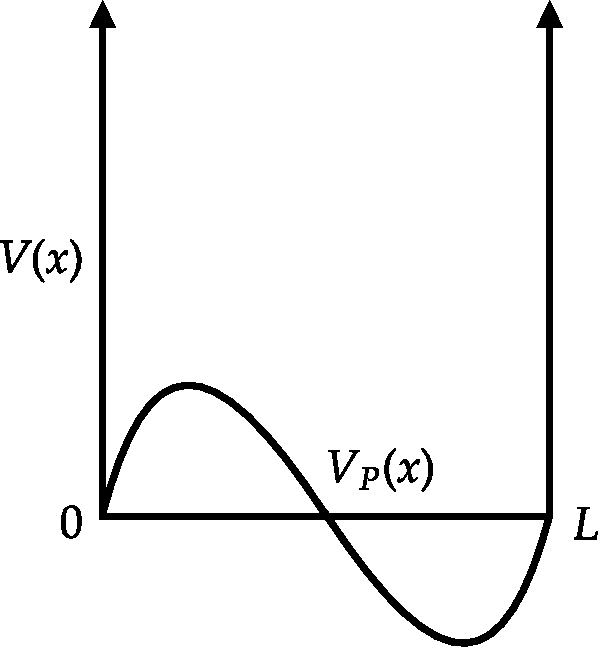
\includegraphics[height=4cm,width=4cm]{diagram-20210824-crop}
		\end{figure}
	\end{minipage}
	\begin{tasks}(2)
		\task[\textbf{A.}] $E^{(1)}=0 ; E^{(2)}<0$
		\task[\textbf{B.}]$E^{(1)}>0 ; E^{(2)}=0$
		\task[\textbf{C.}]$E^{(1)}=0 ; E^{(2)}$ depends on the sign of $V_{0}$
		\task[\textbf{D.}]$E^{(1)}<0 ; E^{(2)}<0$
	\end{tasks}
	\begin{answer}
		$E_{1}^{1}=\frac{2}{L} \int_{0}^{L} V_{0} \sin \frac{2 \pi x}{L} d x=0 ; E_{1}^{2}=\sum_{m \neq 1} \frac{\left|\left\langle\psi_{m}\left|V_{P}\right| \psi_{1}\right\rangle\right|^{2}}{E_{1}-E_{m}} \quad \because E_{1}<E_{m} \text { so } E_{1}^{2}=-v e$\\
		The correct option is \textbf{(a)}	
	\end{answer}
	\begin{minipage}{\textwidth}
		\item An electron with energy $E$ is incident from left on a potential barrier, given by
		$$
		V(x)= \begin{cases}0, & \text { for } x<0 \\ V_{0}, & \text { for } x>0\end{cases}
		$$
		as shown in the figure. For $E<V_{0}$, the space part of the wavefunction for $x>0$ is of the form
		\exyear{GATE 2011}
		\begin{figure}[H]
			\centering
			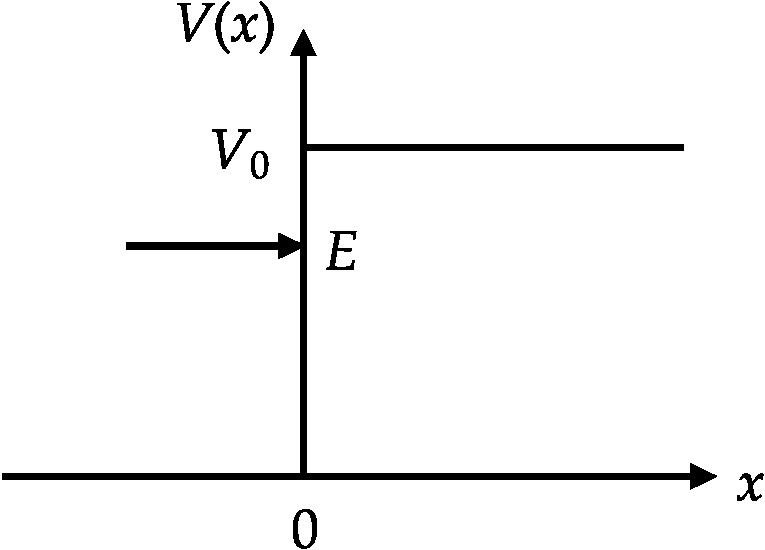
\includegraphics[height=3cm,width=5cm]{diagram-20210824(6)-crop}
		\end{figure}
	\end{minipage}
	\begin{tasks}(2)
		\task[\textbf{A.}] $e^{a x}$
		\task[\textbf{B.}] $e^{-a x}$
		\task[\textbf{C.}] $e^{i a x}$
		\task[\textbf{D.}]$e^{-i a x}$
	\end{tasks}
	\begin{answer}
		$E<V_{0} \text {, so there is decaying wave function. }	$\\
		The correct option is \textbf{(b)}
	\end{answer}
	\begin{minipage}{\textwidth}
		\item A particle of mass $m$ is confined in a two dimensional square well potential of dimension $a$. This potential $V(x, y)$ is given by
		$$
		\begin{aligned}
		V(x, y) &=0 \text { for }-a<x<a \text { and }-a<y<a \\
		&=\infty \text { elsewhere }
		\end{aligned}
		$$
		The energy of the first excited state for this particle is given by,
		\exyear{GATE 2012}
	\end{minipage}
	\begin{tasks}(2)
		\task[\textbf{A.}]$\frac{\pi^{2} \hbar^{2}}{m a^{2}}$
		\task[\textbf{B.}] $\frac{2 \pi^{2} \hbar^{2}}{m a^{2}}$
		\task[\textbf{C.}]$\frac{5 \pi^{2} \hbar^{2}}{8 m a^{2}}$
		\task[\textbf{D.}] $\frac{4 \pi^{2} \hbar^{2}}{m a^{2}}$
	\end{tasks}
	\begin{answer}
		$$E=\left(n_{x}^{2}+n_{y}^{2}\right) \frac{\pi^{2} \hbar^{2}}{2 m(2 a)^{2}}=\left(n_{x}^{2}+n_{y}^{2}\right) \frac{\pi^{2} \hbar^{2}}{8 m a^{2}}=\frac{5 \pi^{2} \hbar^{2}}{8 m a^{2}} \quad \because n_{x}=1, n_{y}=2$$
		The correct option is \textbf{(c)}
	\end{answer}
	\begin{minipage}{\textwidth}
		\item A proton is confined to a cubic box, whose sides have length $10^{-12} \mathrm{~m}$. What is the minimum kinetic energy of the proton? The mass of proton is $1.67 \times 10^{-27} \mathrm{~kg}$ and Planck's constant is $6.63 \times 10^{-34} J_{S}$.
		\exyear{GATE 2013}
	\end{minipage}
	\begin{tasks}(2)
		\task[\textbf{A.}] $1.1 \times 10^{-17} \mathrm{~J}$
		\task[\textbf{B.}] $3.3 \times 10^{-17} \mathrm{~J}$
		\task[\textbf{C.}]$9.9 \times 10^{-17} \mathrm{~J}$
		\task[\textbf{D.}]$6.6 \times 10^{-17} \mathrm{~J}$
	\end{tasks}
	\begin{answer}
		$\frac{3 \pi^{2} \hbar^{2}}{2 m a^{2}}=9.9 \times 10^{-17}$\\
		The correct option is \textbf{(c)}	
	\end{answer}
	\begin{minipage}{\textwidth}
		\item Consider a system of eight non-interacting, identical quantum particles of spin $-\frac{3}{2}$ in a one dimensional box of length $L$. The minimum excitation energy of the system, in units of $\frac{\pi^{2} \hbar^{2}}{2 m L^{2}}$ is
		\exyear{GATE 2015}
	\end{minipage}
	\begin{answer}
		spin $\frac{3}{2} \Rightarrow$ degeneracy $=(2 S+1)=\left(2 \times \frac{3}{2}+1\right)=4$
		$$
		\begin{gathered}
		E_{\text {ground }}=4 \times \frac{\pi^{2} \hbar^{2}}{2 m L^{2}}+4 \times \frac{4 \pi^{2} \hbar^{2}}{2 m L^{2}}=\frac{20 \pi^{2} \hbar^{2}}{2 m L^{2}} \\
		E_{\text {excited }}^{I^{t}}=4 \times \frac{\pi^{2} \hbar^{2}}{2 m L^{2}}+3 \times 4 \frac{\pi^{2} \hbar^{2}}{2 m L^{2}}+1 \times 9 \frac{\pi^{2} \hbar^{2}}{2 m L^{2}}=25 \frac{\pi^{2} \hbar^{2}}{2 m L^{2}}
		\end{gathered}
		$$
		Now minimum excitation energy $\Delta E=E_{\text {excited }}^{I^{s^{\prime}}}-E_{\text {ground }}=25 \frac{\pi^{2} \hbar^{2}}{2 m L^{2}}-20 \frac{\pi^{2} \hbar^{2}}{2 m L^{2}}=5 \frac{\pi^{2} \hbar^{2}}{2 m L^{2}}$	
	\end{answer}
	\begin{minipage}{\textwidth}
		\item A two-dimensional square rigid box of side $L$ contains six non-interacting electrons at $T=0 K .$ The mass of the electron is $m .$ The ground state energy of the system of electrons, in units of $\frac{\pi^{2} \hbar^{2}}{2 m L^{2}}$ is
		\exyear{GATE 2016}
	\end{minipage}
	\begin{answer}
		$ 2 \times \frac{\left(1^{2}+1^{2}\right) \pi^{2} \hbar^{2}}{2 m L^{2}}+4 \times \frac{\left(2^{2}+1^{2}\right) \pi^{2} \hbar^{2}}{2 m L^{2}}=\frac{24 \pi^{2} \hbar^{2}}{2 m L^{2}}$	
	\end{answer}
	\begin{minipage}{\textwidth}
		\item A particle of mass $m$ and energy $E$, moving in the positive $x$ direction, is incident on a step potential at $x=0$, as indicated in the figure. The height of the potential is $V_{0}$, where $V_{0}>E$. At $x=x_{0}$, where $x_{0}>0$, the probability of finding the electron is $\frac{1}{e}$ times the probability of finding it at $x=0$. If $\alpha=\sqrt{\frac{2 m\left(V_{0}-E\right)}{\hbar^{2}}}$, the value of $x_{0}$ is
		\exyear{GATE 2016}
		\begin{figure}[H]
			\centering
			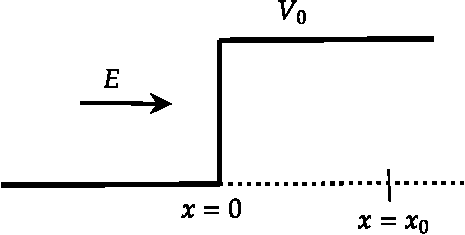
\includegraphics[height=3cm,width=5cm]{gate 5-crop}
		\end{figure}
	\end{minipage}
	\begin{tasks}(2)
		\task[\textbf{A.}] $\frac{2}{\alpha}$
		\task[\textbf{B.}] $\frac{1}{\alpha}$
		\task[\textbf{C.}]$\frac{1}{2 \alpha}$
		\task[\textbf{D.}]$\frac{1}{4 \alpha}$
	\end{tasks}
	\begin{answer}
		$\frac{1}{e}=e^{-2 \alpha x_{0}}=e^{-1}=e^{-2 \alpha x_{0}} \Rightarrow x_{0}=\frac{1}{2 \alpha}$\\
		The correct option is \textbf{(c)}	
	\end{answer}
	\begin{minipage}{\textwidth}
		\item A free electron of energy $1 \mathrm{eV}$ is incident upon a one-dimensional finite potential step of height $0.75 \mathrm{eV}$. The probability of its reflection from the barrier is........... (up to two decimal places).
		\exyear{GATE 2017}
	\end{minipage}
	\begin{answer}
		$R=\left(\frac{\sqrt{E}-\sqrt{E-V_{0}}}{\sqrt{E}+\sqrt{E-V_{0}}}\right)^{2}=\left(\frac{1-\sqrt{0.25}}{1+\sqrt{0.25}}\right)^{2}=\left(\frac{1-0.5}{1+0.5}\right)^{2}=0.11$
	\end{answer}
	\begin{minipage}{\textwidth}
		\item The ground state energy of a particle of mass $m$ in an infinite potential well is $E_{0} .$ It changes to $E_{0}\left(1+\alpha \times 10^{-3}\right)$, when there is a small potential pump of height $V_{0}=\frac{\pi^{2} \hbar^{2}}{50 m L^{2}}$ and width $a=L / 100$, as shown in the figure. The value of $\alpha$ is (up to two decimal places).
		\exyear{GATE 2018}
	\end{minipage}
	\begin{answer}
		$\begin{aligned}
		&\text { Solution: } \alpha_{1}=\left(\frac{L}{2}-\frac{a}{2}\right), \alpha_{2}=\left(\frac{L}{2}+\frac{a}{2}\right), \quad a=\frac{L}{100} \\
		&\qquad \begin{aligned}
		E_{1} &=V_{0} \int_{\alpha_{1}}^{\alpha_{2}}\left(\sqrt{\frac{2}{L}}\right)^{2} \sin ^{2}\left(\frac{\pi x}{L}\right) d x \\
		&=\frac{V_{0}}{L} \int_{\alpha_{1}}^{\alpha_{2}}\left[1-\cos \frac{2 \pi x}{L}\right] d x=\frac{V_{0}}{L}\left[x-\frac{L}{2 \pi} \sin \frac{2 \pi x}{L}\right]_{\alpha_{1}}^{\alpha_{2}}
		\end{aligned}
		\end{aligned}$
		$$
		\begin{aligned}
		&=\frac{V_{0}}{L}\left[a-\frac{L}{2 \pi}\left(\sin \frac{2 \pi(L+a)}{2 L}-\sin \frac{2 \pi(L-a)}{2 L}\right)\right] \\
		&=\frac{V_{0}}{L}\left[\frac{L}{100}-\frac{L}{2 \pi}\left(\sin \left(\pi+\frac{\pi a}{L}\right)-\sin \left(\pi-\frac{\pi a}{L}\right)\right)\right] \\
		&=V_{0}\left[\frac{1}{100}+\frac{1}{2 \pi}(0.0314+0.0314)\right] \\
		&=V_{0} \times 10^{-3}(10+10)=E_{0} \times 10^{-3} \times\left(\frac{20}{25}\right) \Rightarrow \alpha E_{0} \times 10^{-3}=0.81 \times E_{0} \times 10^{-3}
		\end{aligned}
		$$
		Hence, $\alpha=0.81$	
	\end{answer}
	\begin{minipage}{\textwidth}
		\item $ \text { Consider a potential barrier } V(x) \text { of the form: }$
		\begin{figure}[H]
			\centering
			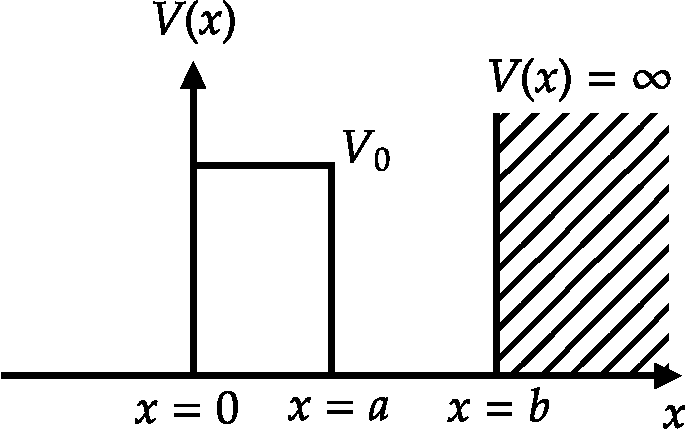
\includegraphics[height=3cm,width=5cm]{diagram-20210825(3)-crop}
		\end{figure}
		where $V_{0}$ is a constant. For particles of energy $E<V_{0}$ incident on this barrier from the left which of the following schematic diagrams best represents the probability density $|\psi(x)|^{2}$ as a function of $x$ ?
		\exyear{GATE 2019}
	\end{minipage}
	\begin{tasks}(2)
		\task[\textbf{A.}]\begin{figure}[H]
			\centering
			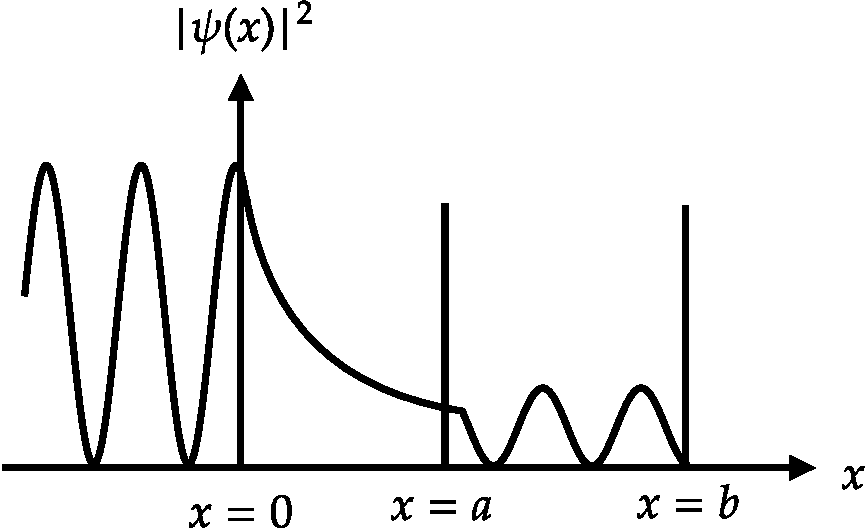
\includegraphics[height=3cm,width=5cm]{diagram-20210825(4)-crop}
		\end{figure}
		\task[\textbf{B.}]\begin{figure}[H]
			\centering
			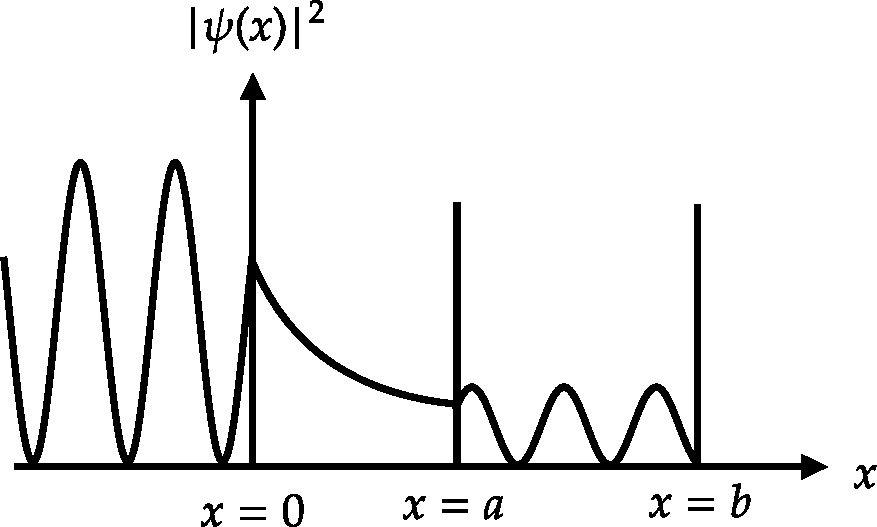
\includegraphics[height=3cm,width=5cm]{diagram-20210825(5)-crop}
		\end{figure}
		\task[\textbf{C.}]\begin{figure}[H]
			\centering
			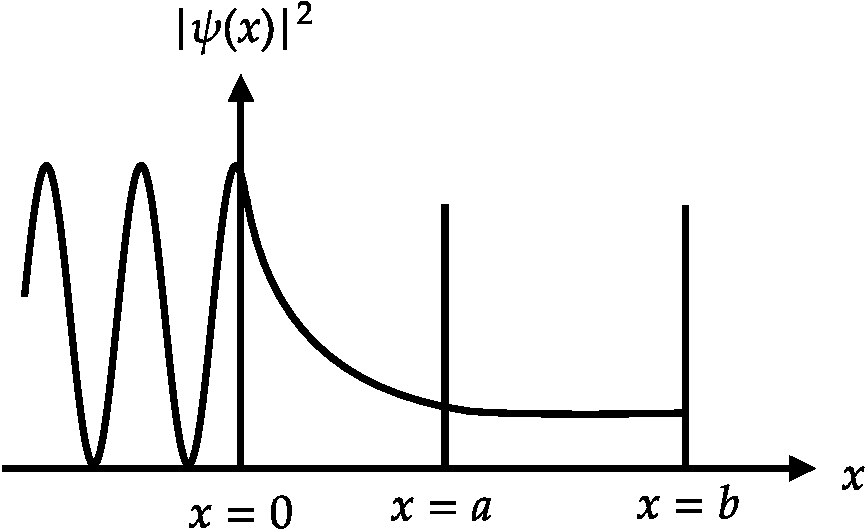
\includegraphics[height=3cm,width=5cm]{diagram-20210825(6)-crop}
		\end{figure}
		\task[\textbf{D.}]\begin{figure}[H]
			\centering
			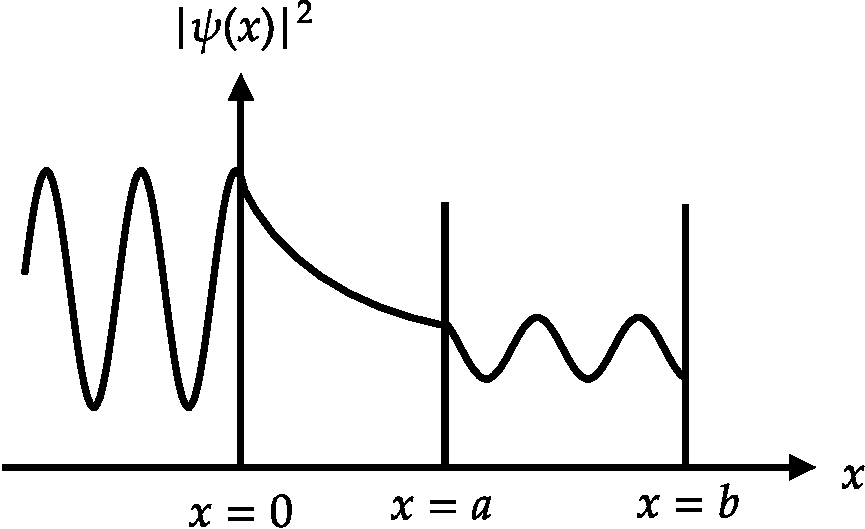
\includegraphics[height=3cm,width=5cm]{diagram-20210825(7)-crop}
		\end{figure}
	\end{tasks}
	\begin{answer}
		The correct option is \textbf{(a)}	
	\end{answer}
\end{enumerate}